% -*- latex -*-
%%%%%%%%%%%%%%%%%%%%%%%%%%%%%%%%%%%%%%%%%%%%%%%%%%%%%%%%%%%%%%%%
%%%%%%%%%%%%%%%%%%%%%%%%%%%%%%%%%%%%%%%%%%%%%%%%%%%%%%%%%%%%%%%%
%%%%
%%%% This text file is part of the source of 
%%%% `Parallel Computing'
%%%% by Victor Eijkhout, copyright 2012/3/4/5
%%%%
%%%% THIS FILE DOES NOT SEEM USED ANYMORE
%%%%
%%%%%%%%%%%%%%%%%%%%%%%%%%%%%%%%%%%%%%%%%%%%%%%%%%%%%%%%%%%%%%%%
%%%%%%%%%%%%%%%%%%%%%%%%%%%%%%%%%%%%%%%%%%%%%%%%%%%%%%%%%%%%%%%%

\Level 0 {Point-to-point communication}

MPI has two types of message passing routines: point-to-point and
collectives. In this section we will discuss point-to-point
communication, which involves the interaction of a unique sender and a
unique receiver. Collectives, which involve all processes in some
joint fashion, will be discussed in the next section.

There is a lot to be said about simple sending and receiving of
data. We will go into three broad categories of operations: blocking
and non-blocking two-sided communication, and the somewhat
more tricky one-sided communication.

Two-sided communication is a little like mail: one party sends data
to another party. The other party can then
be expecting a message from a specified sender or it can be open
to receiving from any source.

An important concept in two-sided communication is that of \indexterm{blocking}.
In a blocking receive, the receiver waits for the message to be deliverd.
Compare it to having to stay at home because FedEx is delivering something
that needs a signature. On the other hand, with a non-blocking receive
you only declare that you are open to receiving. Compare it to installing a mailbox
in your house; you don't wait for the mail, but you'll check it in the evening
when you come home.

One-sided communication is very different in nature. Compare it to leaving your
front-door open and people can bring things to your house, or take them,
without you noticing.

\Level 1 {Concepts: blocking vs non-blocking}
\index{communication!blocking|(textbf}
\index{communication!non-blocking|(textbf}

In two-sided communication, one process issues a send call and the
other a receive call. Life would be easy if the send call put the data
somewhere in the network for the receiving process to find whenever it
gets around to its receive call. This ideal scenario is pictured
figure~\ref{fig:send-ideal}.
\begin{figure}[ht]
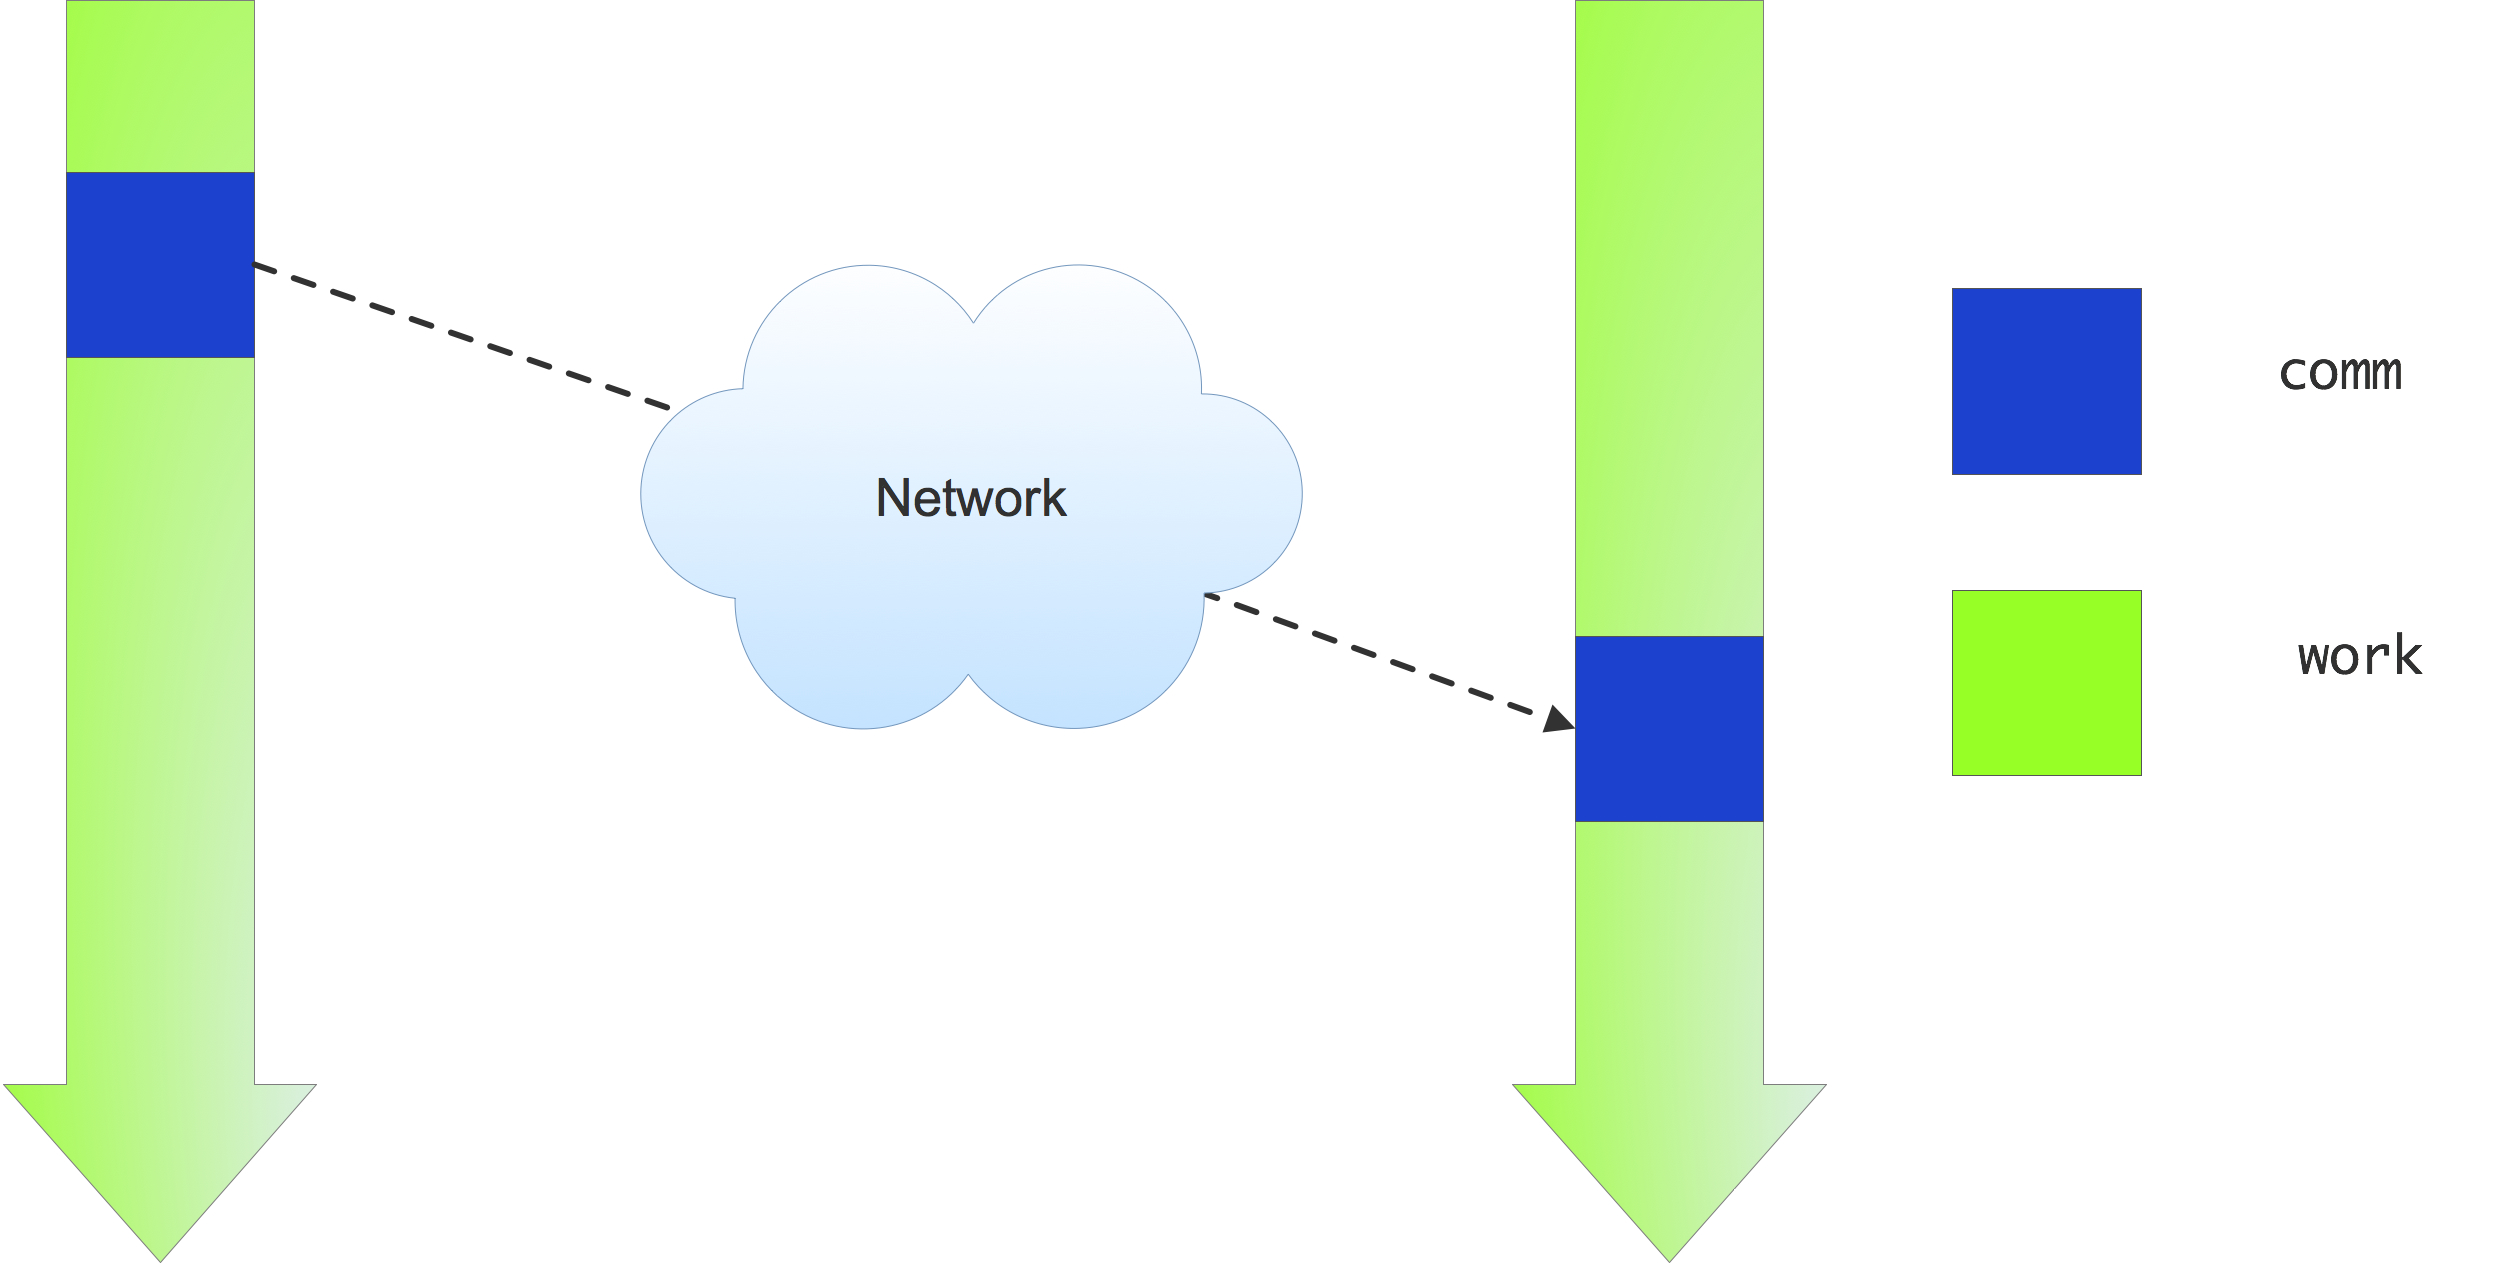
\includegraphics[scale=.1]{graphics/send-ideal}
\caption{Illustration of an ideal send-receive interaction}
\label{fig:send-ideal}
\end{figure}

The above ideal scenario is not realistic: it assumes that somewhere
in the network there is buffer capacity for all messages that are in
transit. Since this message volume can be large, we have to worry
explicitly about management of send and receive \indexterm{buffers}.

The easiest scenario is that the sending process keeps the message
data in a local data structure until the receiving process has indicated
that it is ready to receive it. This is pictured in
figure~\ref{fig:blockingnonblocking} on the left.
\begin{figure}[ht]
\leavevmode
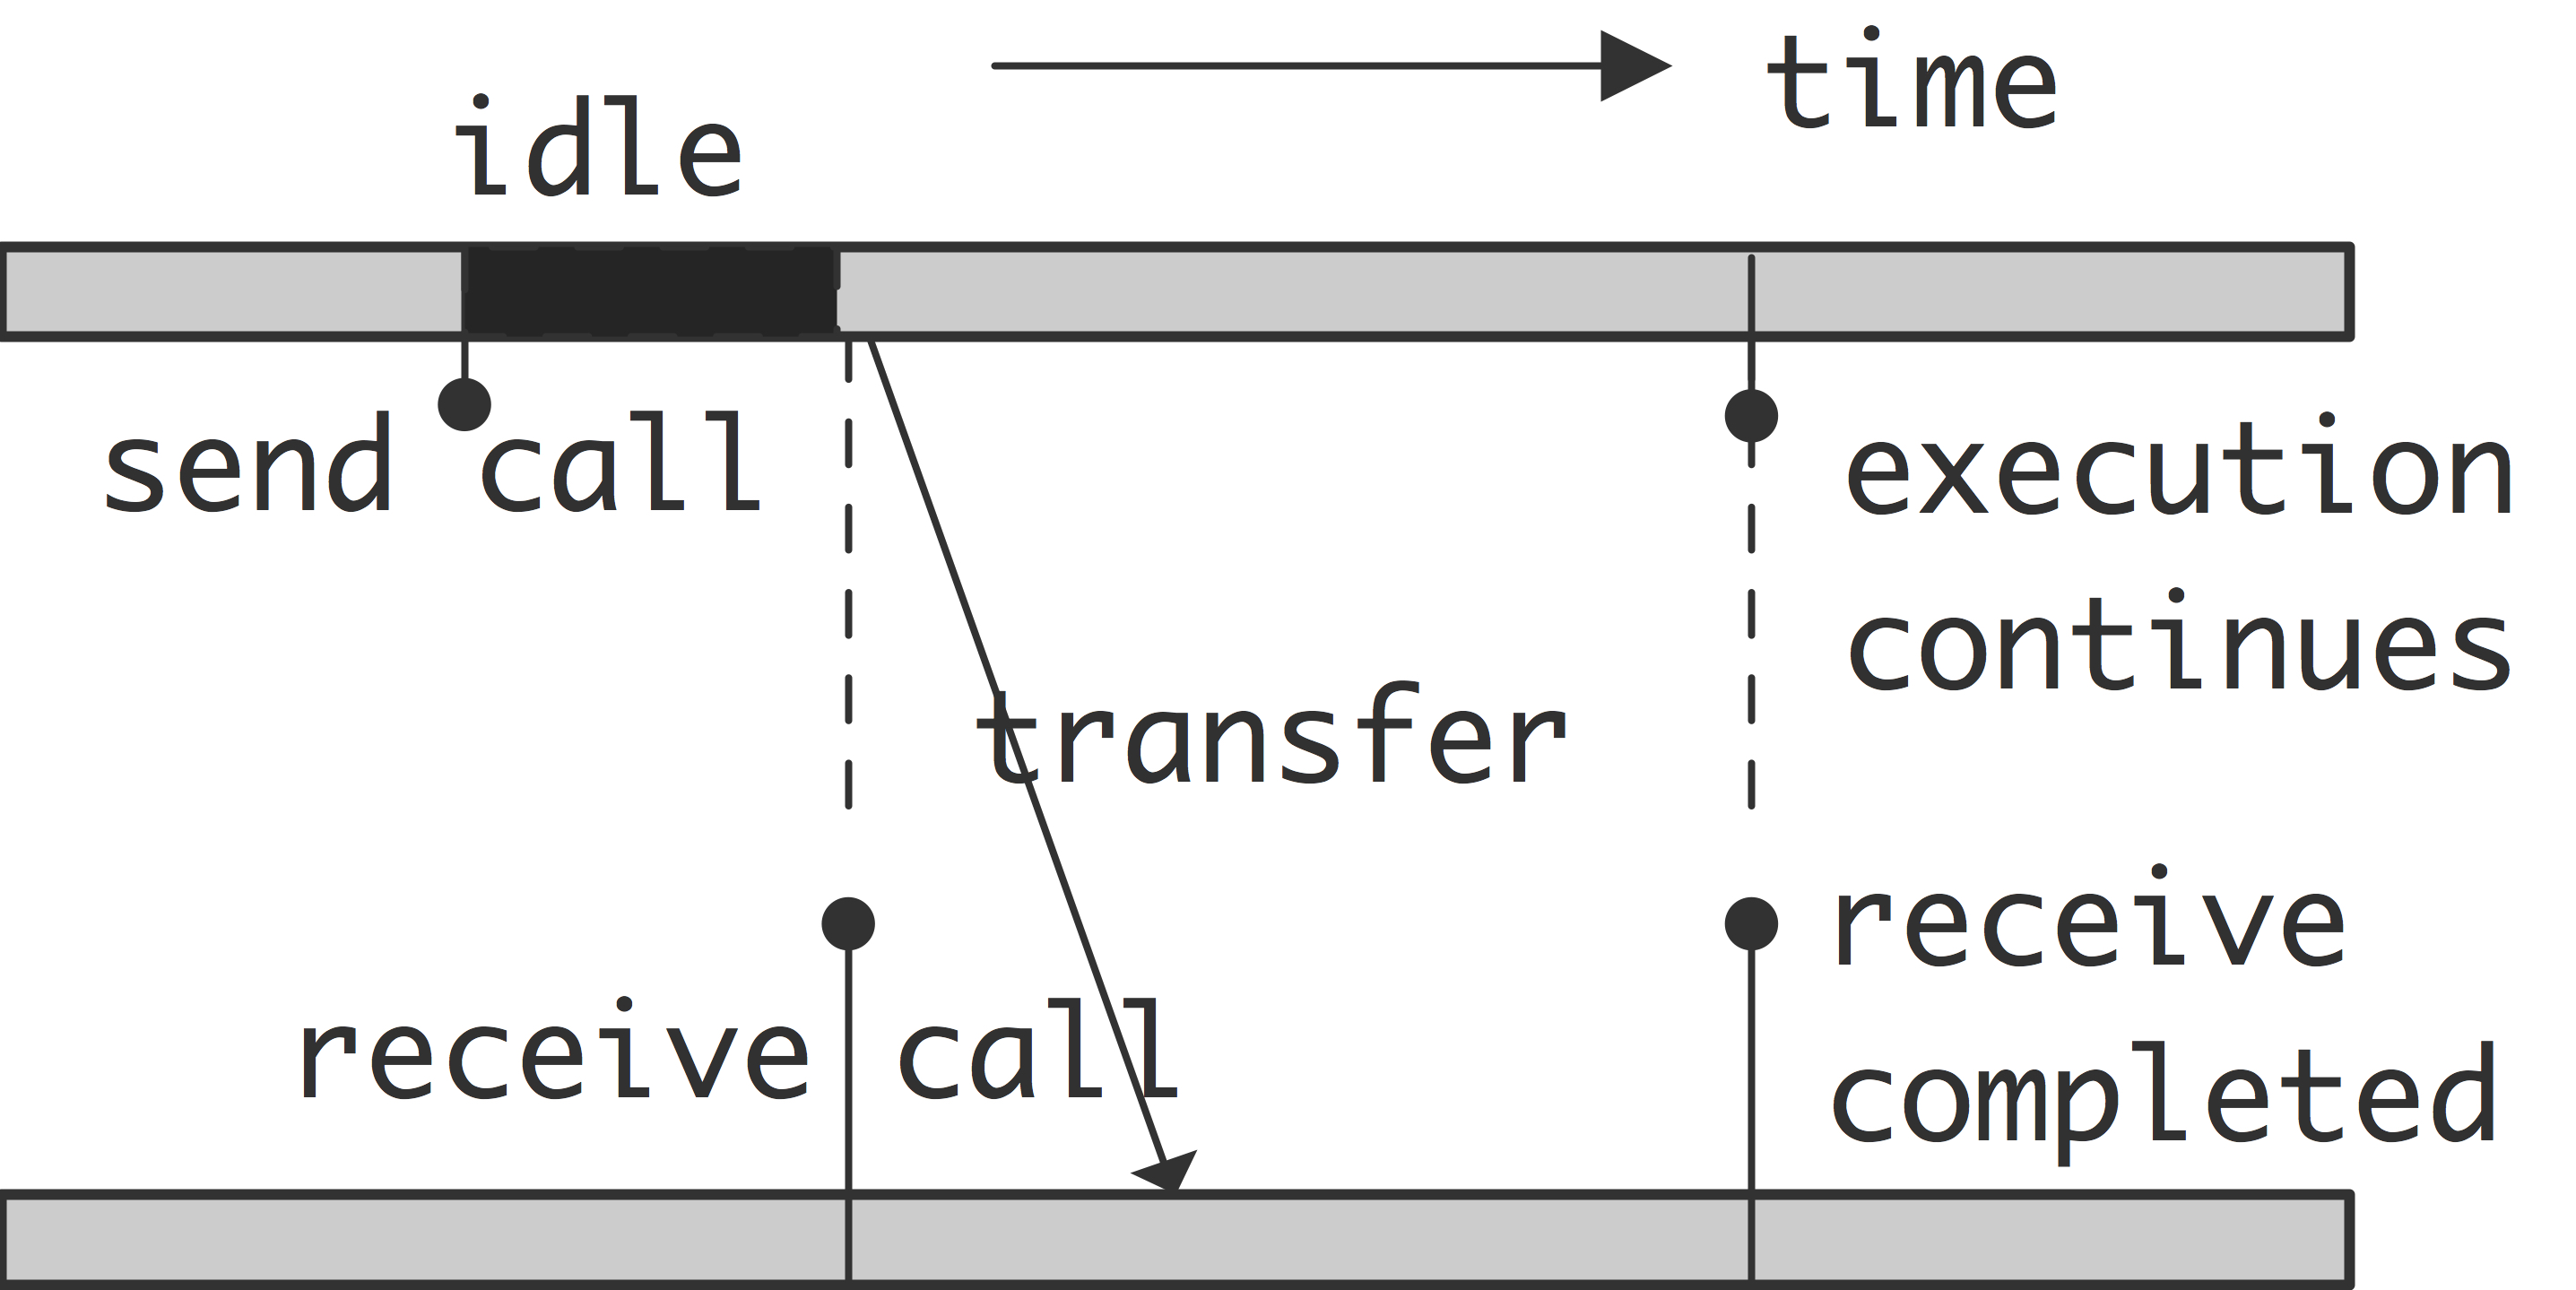
\includegraphics[scale=.08]{blockingsend}
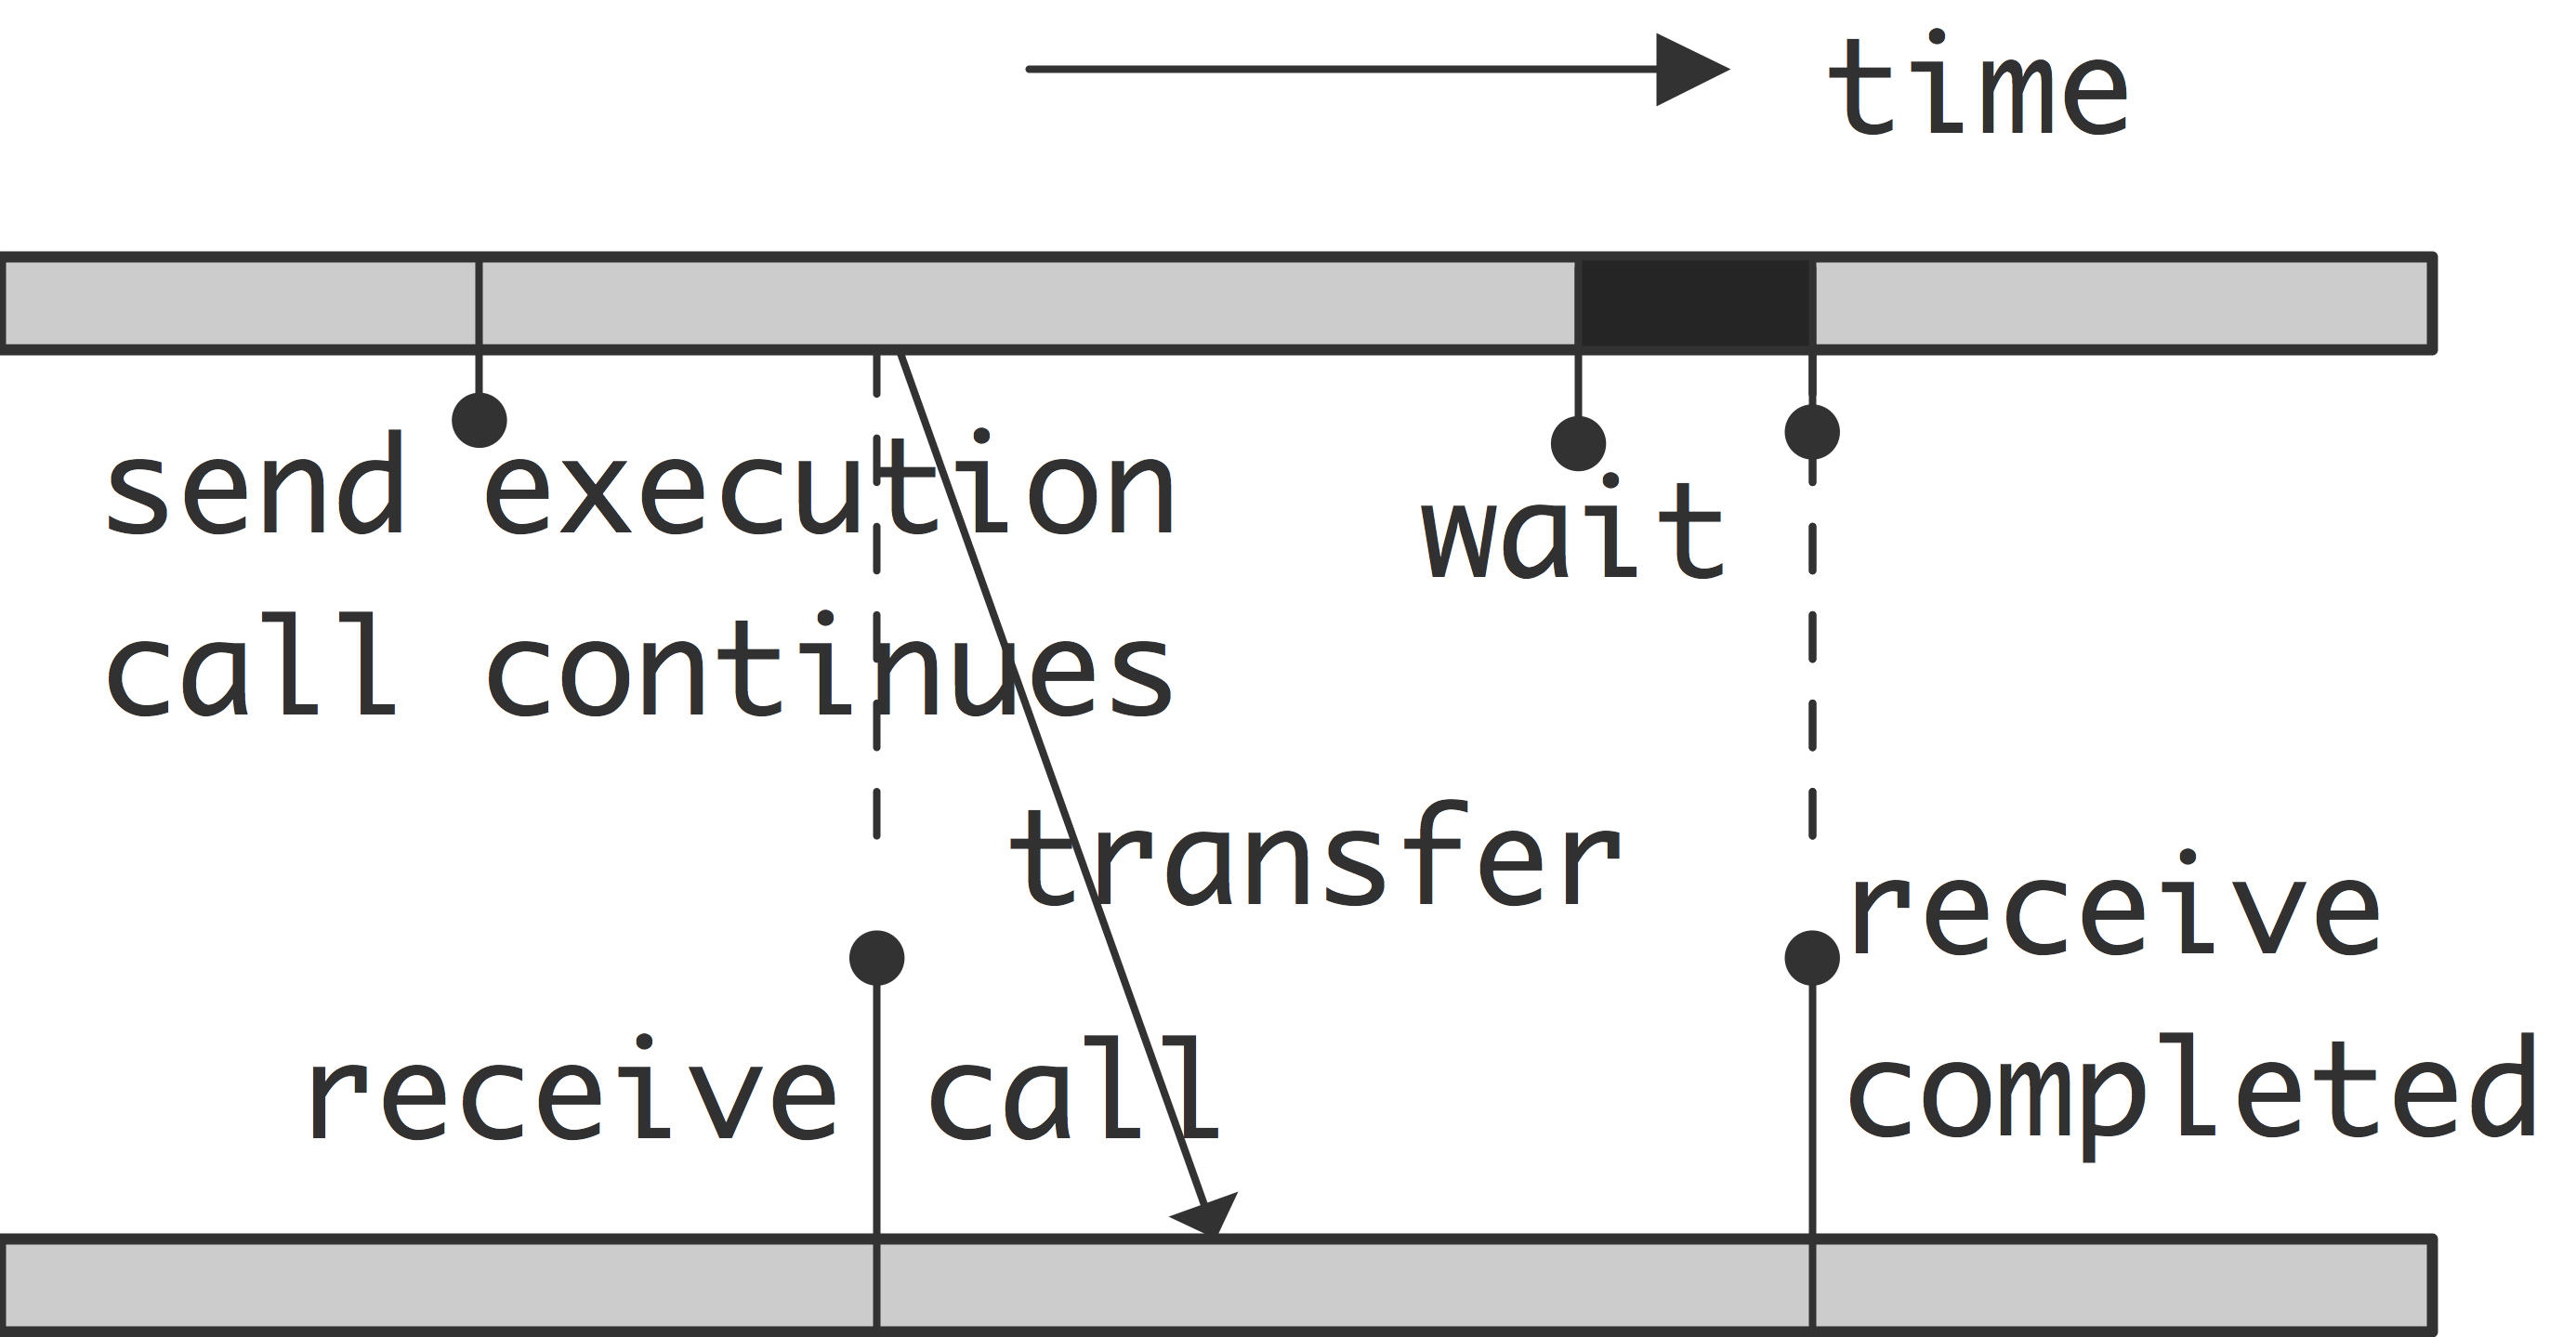
\includegraphics[scale=.08]{nonblockingsend}
\caption{Blocking (left) and nonblocking (right) transfer}
\label{fig:blockingnonblocking}
\end{figure}
%
This is known as \emph{blocking} communication: a process that issues
a send or receive call will then block until the corresponding receive
or send call is successfully concluded. 
Blocking communication can be inefficient if processors are not
perfectly in sync, or if messages are large and transfer takes
a lot of time. In both cases the communication adds \indexterm{overhead}
to the parallel running time, limiting the attained speedup
from running in parallel. The first scenario, where the idle time (see the picture)
is the cause of the overhead, is said to be caused to \indexterm{load imbalance}:
if the sender had had more work, or the receiver less, the idle time
could have been eliminated.

However, there is a different way of dealing with communication overhead.
It would be better if send call does not wait for the corresponding receive,
but only sets aside the data for the system to transfer it, 
while the user program continues. This is known as \emph{non-blocking}
communication, illustrated in figure~\ref{fig:nonblocking}.

\index{communication!non-blocking|)}
\index{communication!blocking|)}

\Level 1 {Blocking communication}
\index{communication!two-sided|(}
\index{communication!blocking|(textbf}
\commandref{blocking}

Above we signalled a first problem with blocking communication:
if your
processes are not perfectly synchronized your performance may degrade
because processes spend time waiting for each other;
see~\HPSCref{sec:load}. 
But there is a more insidious, more serious problem.
Suppose two process need to exchange data, and consider the following
pseudo-code, which purports to exchange data between processes 0 and~1:
\begin{verbatim}
other = 1-mytid; /* if I am 0, other is 1; and vice versa */
send(target=other);
receive(source=other);
\end{verbatim}
Imagine that the two processes execute this code. They both issue the
send call\ldots\ and then can't go on, because they are both waiting
for the other to issue a receive call. This is known
as \indexterm{deadlock}.

Formally you can describe deadlock as follows. Draw up a graph where
every process is a node, and draw a directed arc from process~A to~B if
A is waiting for~B. There is deadlock if this directed graph has a
loop.

The solution to the deadlock in the above example
is to first do the send from 0 to~1, and then from 1 to~0 (or the other way around). So the code would look like:
\begin{verbatim}
if ( /* I am processor 0 */ ) {
  send(target=other);
  receive(source=other);
} else {
  receive(source=other);
  send(target=other);
}
\end{verbatim}

There is even a third, even more subtle problem with blocking
communication. Consider the scenario where every processor needs to
pass data to its successor, that is, the processor with the next
higher rank. The basic idea would be to first send to your successor,
then receive from your predecessor. Since the last processor does not
have a successor it skips the send, and likewise the first processor
skips the receive. The pseudo-code looks like:
\begin{verbatim}
successor = mytid+1; predecessor = mytid-1;
if ( /* I am not the last processor */ )
  send(target=successor);
if ( /* I am not the first processor */ )
  receive(source=predecessor)
\end{verbatim}
This code does not deadlock. All processors but the last one block on
the send call, but the last processor executes the receive call. Thus,
the processor before the last one can do its send, and subsequently
continue to its receive, which enables another send, et cetera.

In one way this code does what you intended to do:
it will terminate (instead of hanging forever on a
deadlock) and exchange data the right way. However, the execution
now suffers from \indextermsub{unexpected}{serialization}: only
one processor is active at any time, so what should have been a
\begin{figure}[ht]
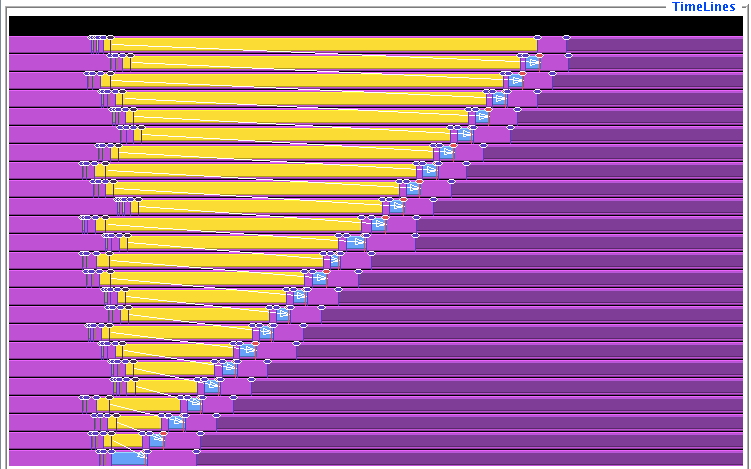
\includegraphics[scale=.4]{graphics/linear-serial}
\caption{Trace of a simple send-recv code}
\label{fig:serialization}
\end{figure}
parallel operation becomes a sequential one. This is illustrated in
figure~\ref{fig:serialization}.
\begin{exercise}
\label{ex:linear-sequential}
  Modify your earlier code, run it and reproduce the trace output 
  of figure~\ref{fig:serialization}. See chapter~\ref{tut:tau}
  on how to use the TAU utility.
\end{exercise}
It is possible to orchestrate your processes to get an efficient and
deadlock-free execution, but doing so is a bit cumbersome.
There are better solutions which we will
explore next.

\begin{exercise}
  The above solution treated every processor equally. Can you come up
  with a solution that uses blocking sends and receives, but does not
  suffer from the serialization behaviour?
\end{exercise}

\begin{comment}
  \begin{exercise}
    There are rare circumstances where you actually want this serial
    behaviour. Recall from exercise~\ref{ex:hello-world-zero} that
    output from processes is not automatically serialized. Take your
    code from that exercise, and use the serialization behaviour your
    observed to force the processes to output their print statements in
    sequence.
  \end{exercise}
\end{comment}

Above, you saw a code fragment with a conditional send:
\begin{verbatim}
MPI_Comm_rank( .... &mytid );
successor = mytid+1
if ( /* I am not the last processor */ )
  send(target=successor);
\end{verbatim}
MPI allows for the following variant which makes the code slightly 
more homogeneous:
\begin{verbatim}
MPI_Comm_rank( .... &mytid );
if ( /* I am not the last processor */ )
  successor = mytid+1
else
  successor = MPI_PROC_NULL;
send(target=successor);
\end{verbatim}
where the send call is executed by all processors.
All processors but the last one send to their neighbour; the target value
of \indexmpidef{MPI_PROC_NULL} for the last processor
means a `send to the null processor':  no actual send is done. 
The null processor
value is also of use with the \indexmpishow{MPI_Sendrecv} call;
section~\ref{sec:send-recv}

\Level 2 {Deadlock-free blocking communication}
\commandref{send-recv}

Above you saw that with blocking sends the precise ordering of the
send and receive calls is crucial. Use the wrong ordering and you get
either deadlock, or something that is not efficient at all in
parallel. MPI has a way out of this problem that is sufficient for
many purposes: the combined send/recv call\indexmpishow{MPI_Sendrecv}
\begin{verbatim}
MPI_Sendrecv( /* send data */ ....
               /* recv data */ .... );
\end{verbatim}
This call makes it easy to exchange data between two processors: both
specify the other as both target and source. However, there need not
be any such relation between target and source: it is possible to
receive from a predecessor in some ordering, and send to a successor
in that ordering; see figure~\ref{fig:sendrecv}.
\begin{figure}[ht]
\begin{lulu}
    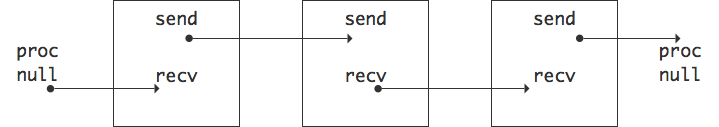
\includegraphics[scale=.6]{sendrecv-actual}
\end{lulu}
\begin{notlulu}
    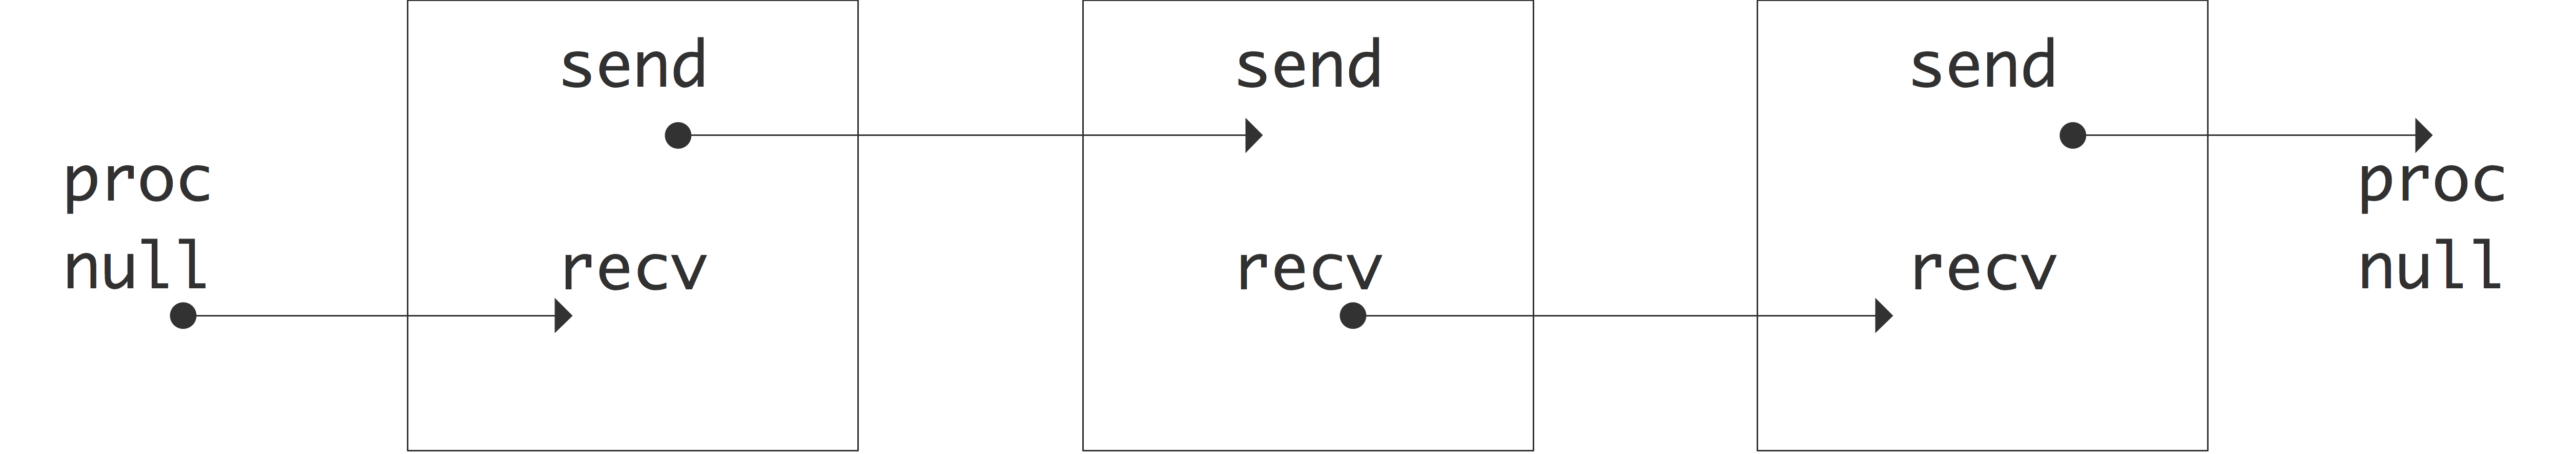
\includegraphics[scale=.09]{sendrecv}
\end{notlulu}
  \caption{An MPI Sendrecv call}
  \label{fig:sendrecv}
\end{figure}
Above you saw some examples that had most processors doing both a send and
a receive, but some only a send or only a receive. You can still use
\n{MPI_Sendrecv} in this call if you use \indexmpishow{MPI_PROC_NULL} for
the unused source or target argument.

If the send and receive buffer have the same size, the routine
\indexmpishow{MPI_Sendrecv_replace} will do an in-place replacement.

\begin{exercise}
\label{ex:linear-sendrecv}
  Take your code from exercise~\ref{ex:linear-sequential}
  and rewrite it to use the \n{MPI_Sendrecv} call. Run it and
  produce a trace output. Do you see the serialization behaviour
  of your earlier code?
\end{exercise}

\begin{wrapfigure}{r}{3.5in}
  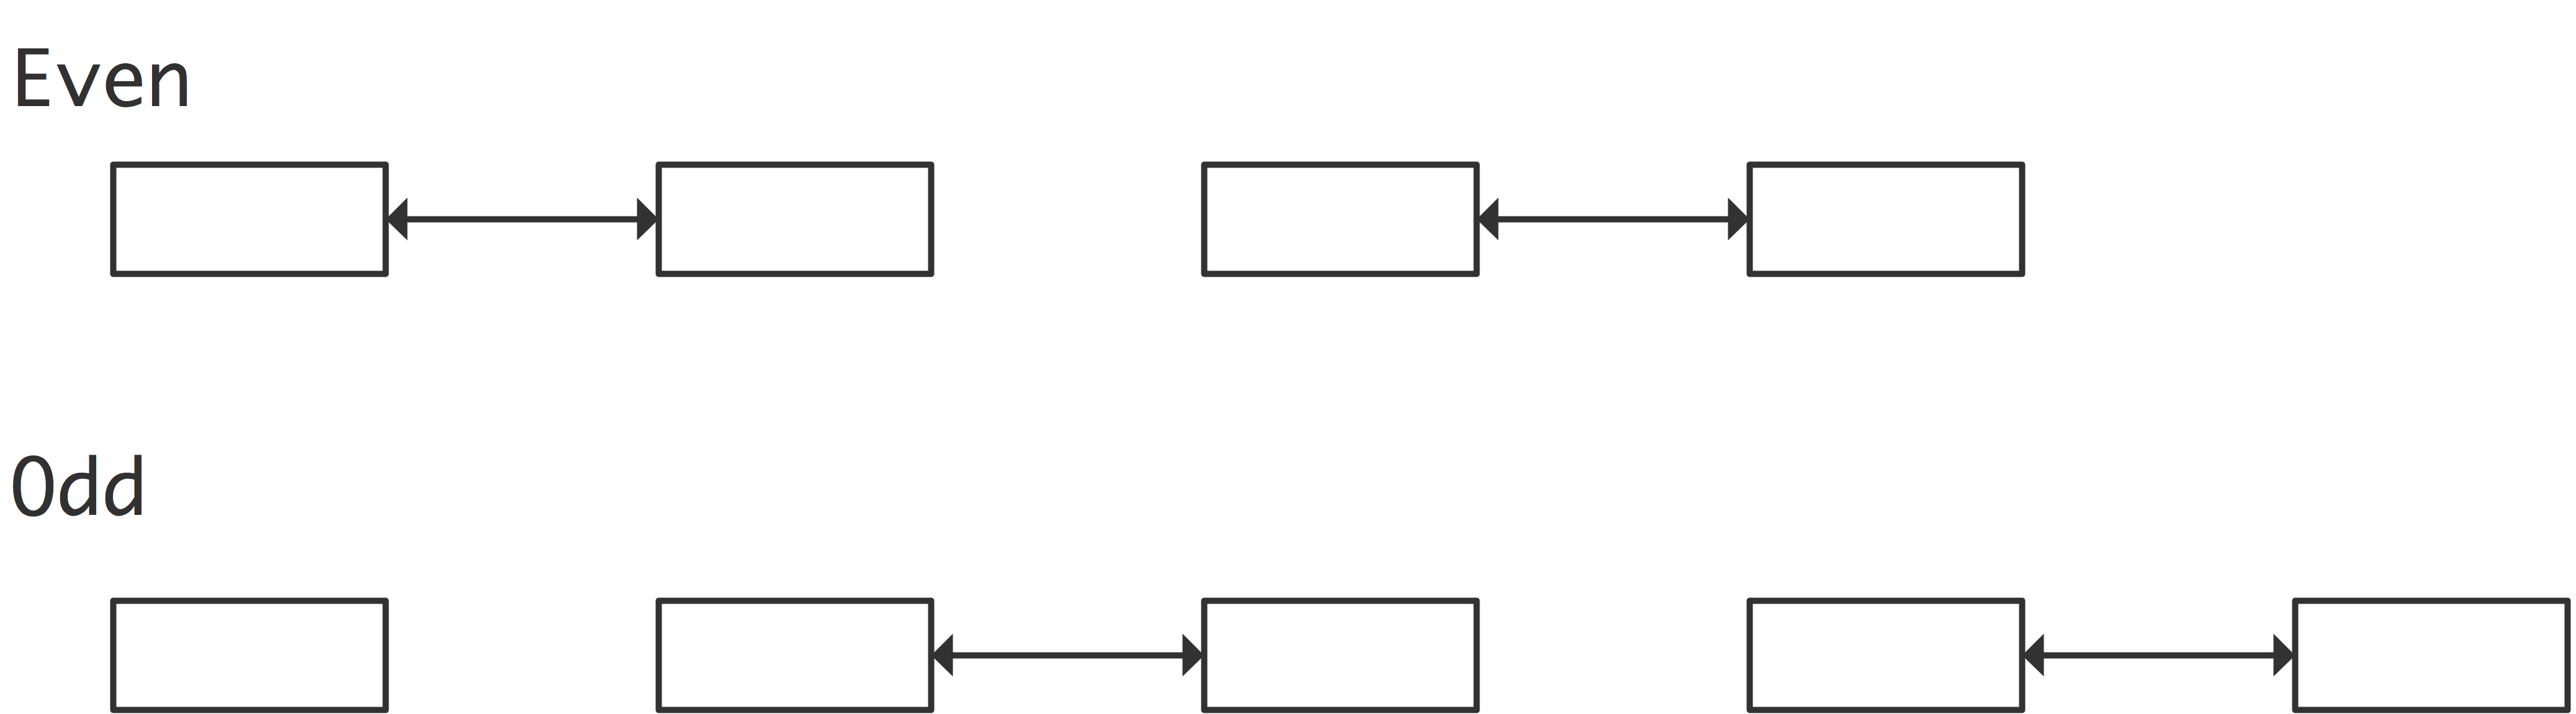
\includegraphics[scale=.06]{swapsort}
\end{wrapfigure}
%
The following exercise lets you implement a sorting algorithm with the send-receive call.
\begin{exercise}
  \label{ex:exchange-sort}
  A very simple sorting algorithm is \indextermsub{exchange}{sort}:
  pairs of processors compare data, and if necessary exchange. The
  elementary step is called a \indexterm{compare-and-swap}: in a pair
  of processors each sends their data to the other; one keeps the
  minimum values, and the other the maximum.
  For simplicity, in this exercise we give each processor just a single number.

  The exchange sort algorithm is split in even and odd stages:
  \begin{itemize}
  \item In the even stage, processors $2i$ and $2i+1$ compare and swap data;
  \item In the odd stage, processors $2i+1$ and $2i+2$ compare and swap.
  \end{itemize}
  You need to repeat this $P/2$ times, where $P$~is the number of processors.

  Use \n{MPI_PROC_NULL} for the edge cases.
\end{exercise}

\Level 2 {Wildcards in the receive call}
\commandref{mpi-source}

In some applications it makes sense that a message can come from 
one of a number of processes. In this case, it is possible to specify
\indexmpishow{MPI_ANY_SOURCE} as the source. To find out where the message actually
came from, you would use the \indexmpishow{MPI_SOURCE} field of the status object
that is delivered by \n{MPI_Recv} or the \n{MPI_Wait...} call after an \n{MPI_Irecv}.
\begin{verbatim}
MPI_Recv(recv_buffer+p,1,MPI_INT, MPI_ANY_SOURCE,0,comm,
         &status);
sender = status.MPI_SOURCE;
\end{verbatim}

There are various scenarios where receiving from `any source' makes sense.
One is that of the \indexterm{master-worker model}. The master task would first send
data to the worker tasks, then issues a blocking wait for the data of whichever process
finishes first.

If a processor is expecting more than one messsage from a single other processor,
message tags are used to distinguish between them. In that case,
a value of \indexmpishow{MPI_ANY_TAG} can be used, and the actual tag
of a message can be retrieved with
\begin{verbatim}
int tag = status.MPI_TAG;
\end{verbatim}

If the amount of data received is not known a~priori, the amount received
can be found as
\begin{verbatim}
MPI_Get_count(&recv_status,MPI_INT,&recv_count);
\end{verbatim}

% MPI_Probe

\index{communication!blocking|)}

\Level 1 {Non-blocking communication}
\commandref{nonblocking}
\index{communication!non-blocking|(textbf}

In the previous section you saw that blocking communication makes
programming tricky if you want to avoid deadlock and performance
problems. The main advantage of these routines is that you have full
control about where the data is: if the send call returns
the data has been successfully received, and the send buffer can be used for
other purposes or de-allocated.  

By constrast, the non-blocking calls \indexmpishow{MPI_Isend} and \indexmpishow{MPI_Irecv}
do not wait for their counterpart: in effect they tell the runtime
system `here is some data and please send it as follows' or `here is
some buffer space, and expect such-and-such data to
come'. 
This is illustrated in figure~\ref{fig:send-nonblocking}.

While the use of non-blocking routines prevents deadlock, it
introduces two new problems:
\begin{enumerate}
\item When the send call returns, the actual send may not have been executed,
  so the send buffer may not be safe to
  overwrite. When the recv call returns, you do not know for sure that
  the expected data is in it. Thus, you need a mechanism to make sure
  that data was actually sent or received.
\item With a blocking send call, you could repeatedly fill the send
  buffer and send it off.
\begin{verbatim}
double *buffer;
for ( ... p ... ) {
   buffer = // fill in the data
   MPI_Send( buffer, ... /* to: */ p );
\end{verbatim}
  To send multiple messages with non-blocking calls
  you have to allocate multiple buffers.
\begin{verbatim}
double **buffers;
for ( ... p ... ) {
   buffers[p] = // fill in the data
   MPI_Send( buffers[p], ... /* to: */ p );
\end{verbatim}
\end{enumerate}

For the first problem, MPI has two types of
routines. The \indexmpishow{MPI_Wait...} calls are blocking: when you issue
such a call, your execution will wait until the specified requests
have been completed. A~typical way of using them is:
\begin{verbatim}
// start non-blocking communication
MPI_Isend( ... ); MPI_Irecv( ... );
// do work that does not depend on incoming data
....
// wait for the Isend/Irecv calls to finish
MPI_Wait( ... );
// now do the work that absolutely needs the incoming data
....
\end{verbatim}

\Level 2 {Wait calls}

There are several wait calls:
\begin{itemize}
\item \indexmpishow{MPI_Wait} waits for a a single request. If you are
  indeed waiting for a single nonblocking communication to complete,
  this is the right routine. If you are waiting for multiple requests
  you could call this routine in a loop. 
\begin{verbatim}
for (p=0; p<nrequests ; p++)
  MPI_Wait(request[p],&(status[p]));
\end{verbatim}
  However, this would be inefficient if the first request is fulfilled much later than 
  the others: your waiting process would have lots of idle time. In that case,
  use one of the following routines.
\item \indexmpishow{MPI_Waitall} allows you to wait for a number of
  requests, and it does not matter in what sequence they are
  satisfied. Using this routine is easier to code than the loop above,
  and it could be more efficient.
\item The `waitall' routine is good if you need all nonblocking
  communications to be finished before you can proceed with the rest
  of the program. However, sometimes it is possible to take action as
  each request is satisfied. In that case you could use
  \indexmpishow{MPI_Waitany} and write:
\begin{verbatim}
for (p=0; p<nrequests; p++) {
  MPI_Waitany(nrequests,request_array,&index,&status);
  // operate on buffer[index]
}
\end{verbatim}
  Note that this routine takes a single status argument, passed by reference,
  and not an array of statuses!
\item \indexmpishow{MPI_Waitsome} is very much like \n{Waitany},
  except that it returns multiple numbers, if multiple requests are
  satisfied. Now the status argument is an array of \n{MPI_Status} objects.
\end{itemize}

Figure~\ref{fig:jump-nonblock} shows the trace of a non-blocking execution
using \n{MPI_Waitall}.
\begin{figure}[ht]
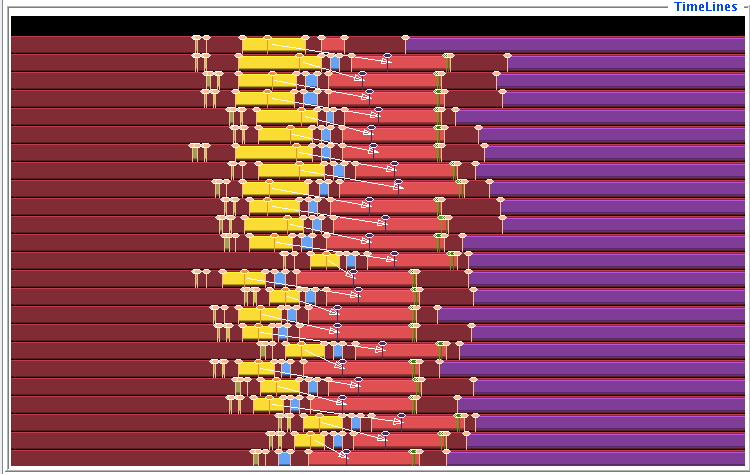
\includegraphics[scale=.4]{graphics/linear-nonblock}
\caption{A trace of a nonblocking send between neighbouring processors}
\label{fig:jump-nonblock}
\end{figure}

The \n{MPI_Wait...} routines are blocking. Thus, they are a good solution if 
the receiving process can not do anything until the data 
(or at least \emph{some} data) is actually received.
The \mpiindexshow{MPI_Test....} calls are themselves non-blocking: they
test for whether one or more requests have been
fullfilled, but otherwise immediately return.
This can be used in the
\indexterm{master-worker model}: the master process creates tasks, and
sends them to whichever worker process has finished its work,
but while it waits for the workers it can itself do useful work.
Pseudo-code:
\begin{verbatim}
while ( not done ) {
  // create new inputs for a while
  ....
  // see if anyone has finished
  MPI_Test( .... &index, &flag );
  if ( flag ) {
    // receive processed data and send new
}
\end{verbatim}

\begin{exercise}
  Read section~\HPSCref{sec:pspmvp} and give pseudo-code for the
    distributed sparse matrix-vector product using the above idiom for
    using \n{MPI_Test...} calls. Discuss the advantages and
    disadvantages of this approach. The answer is not going to be
    black and white: discuss when you expect which approach to be
    preferable.
\end{exercise}

\Level 2 {Test and Probe}

\Level 2 {Overlap of computation and communication}

Non-blocking routines have long held the promise of letting a
program \emph{overlap its computation and
communication}\index{communication!overlap with computation}.  The
idea was that after posting the non-blocking calls the program could
proceed to do non-communication work, while another part of the system
would take care of the communication. Unfortunately, a~lot of this 
communication involved activity in user space, so the solution would have
been to let it be handled by a separate thread. Until recently, processors
were not efficient at doing such multi-threading, so true overlap 
stayed a promise for the future.

\Level 2 {More about non-blocking}

Above we used \n{MPI_Irecv}, but we could have used the \n{MPI_Recv}
routine.  There is nothing special about a non-blocking or synchronous
message once it arrives; the \n{MPI_Recv} call can match any of the
send routines you have seen so far (but not \n{MPI_Sendrecv}).

\Level 1 {Synchronous and asynchronous communication}

\index{communication!synchronous|(textbf}
\index{communication!asynchronous|(textbf}

It is easiest to think of blocking as a form of synchronization with
the other process, but that is not quite true. Synchronization is a
concept in itself, and we talk about \emph{synchronous} communication
if there is actual coordination going on with the other process,
and \emph{asynchronous} communication if there is not. Blocking then
only refers to the program waiting until the user data is safe
to reuse; in the synchronous case a blocking call means that the data
is indeed transferred, in the asynchronous case it only means that the
data has been transferred to some system buffer.
%
\begin{figure}[ht]
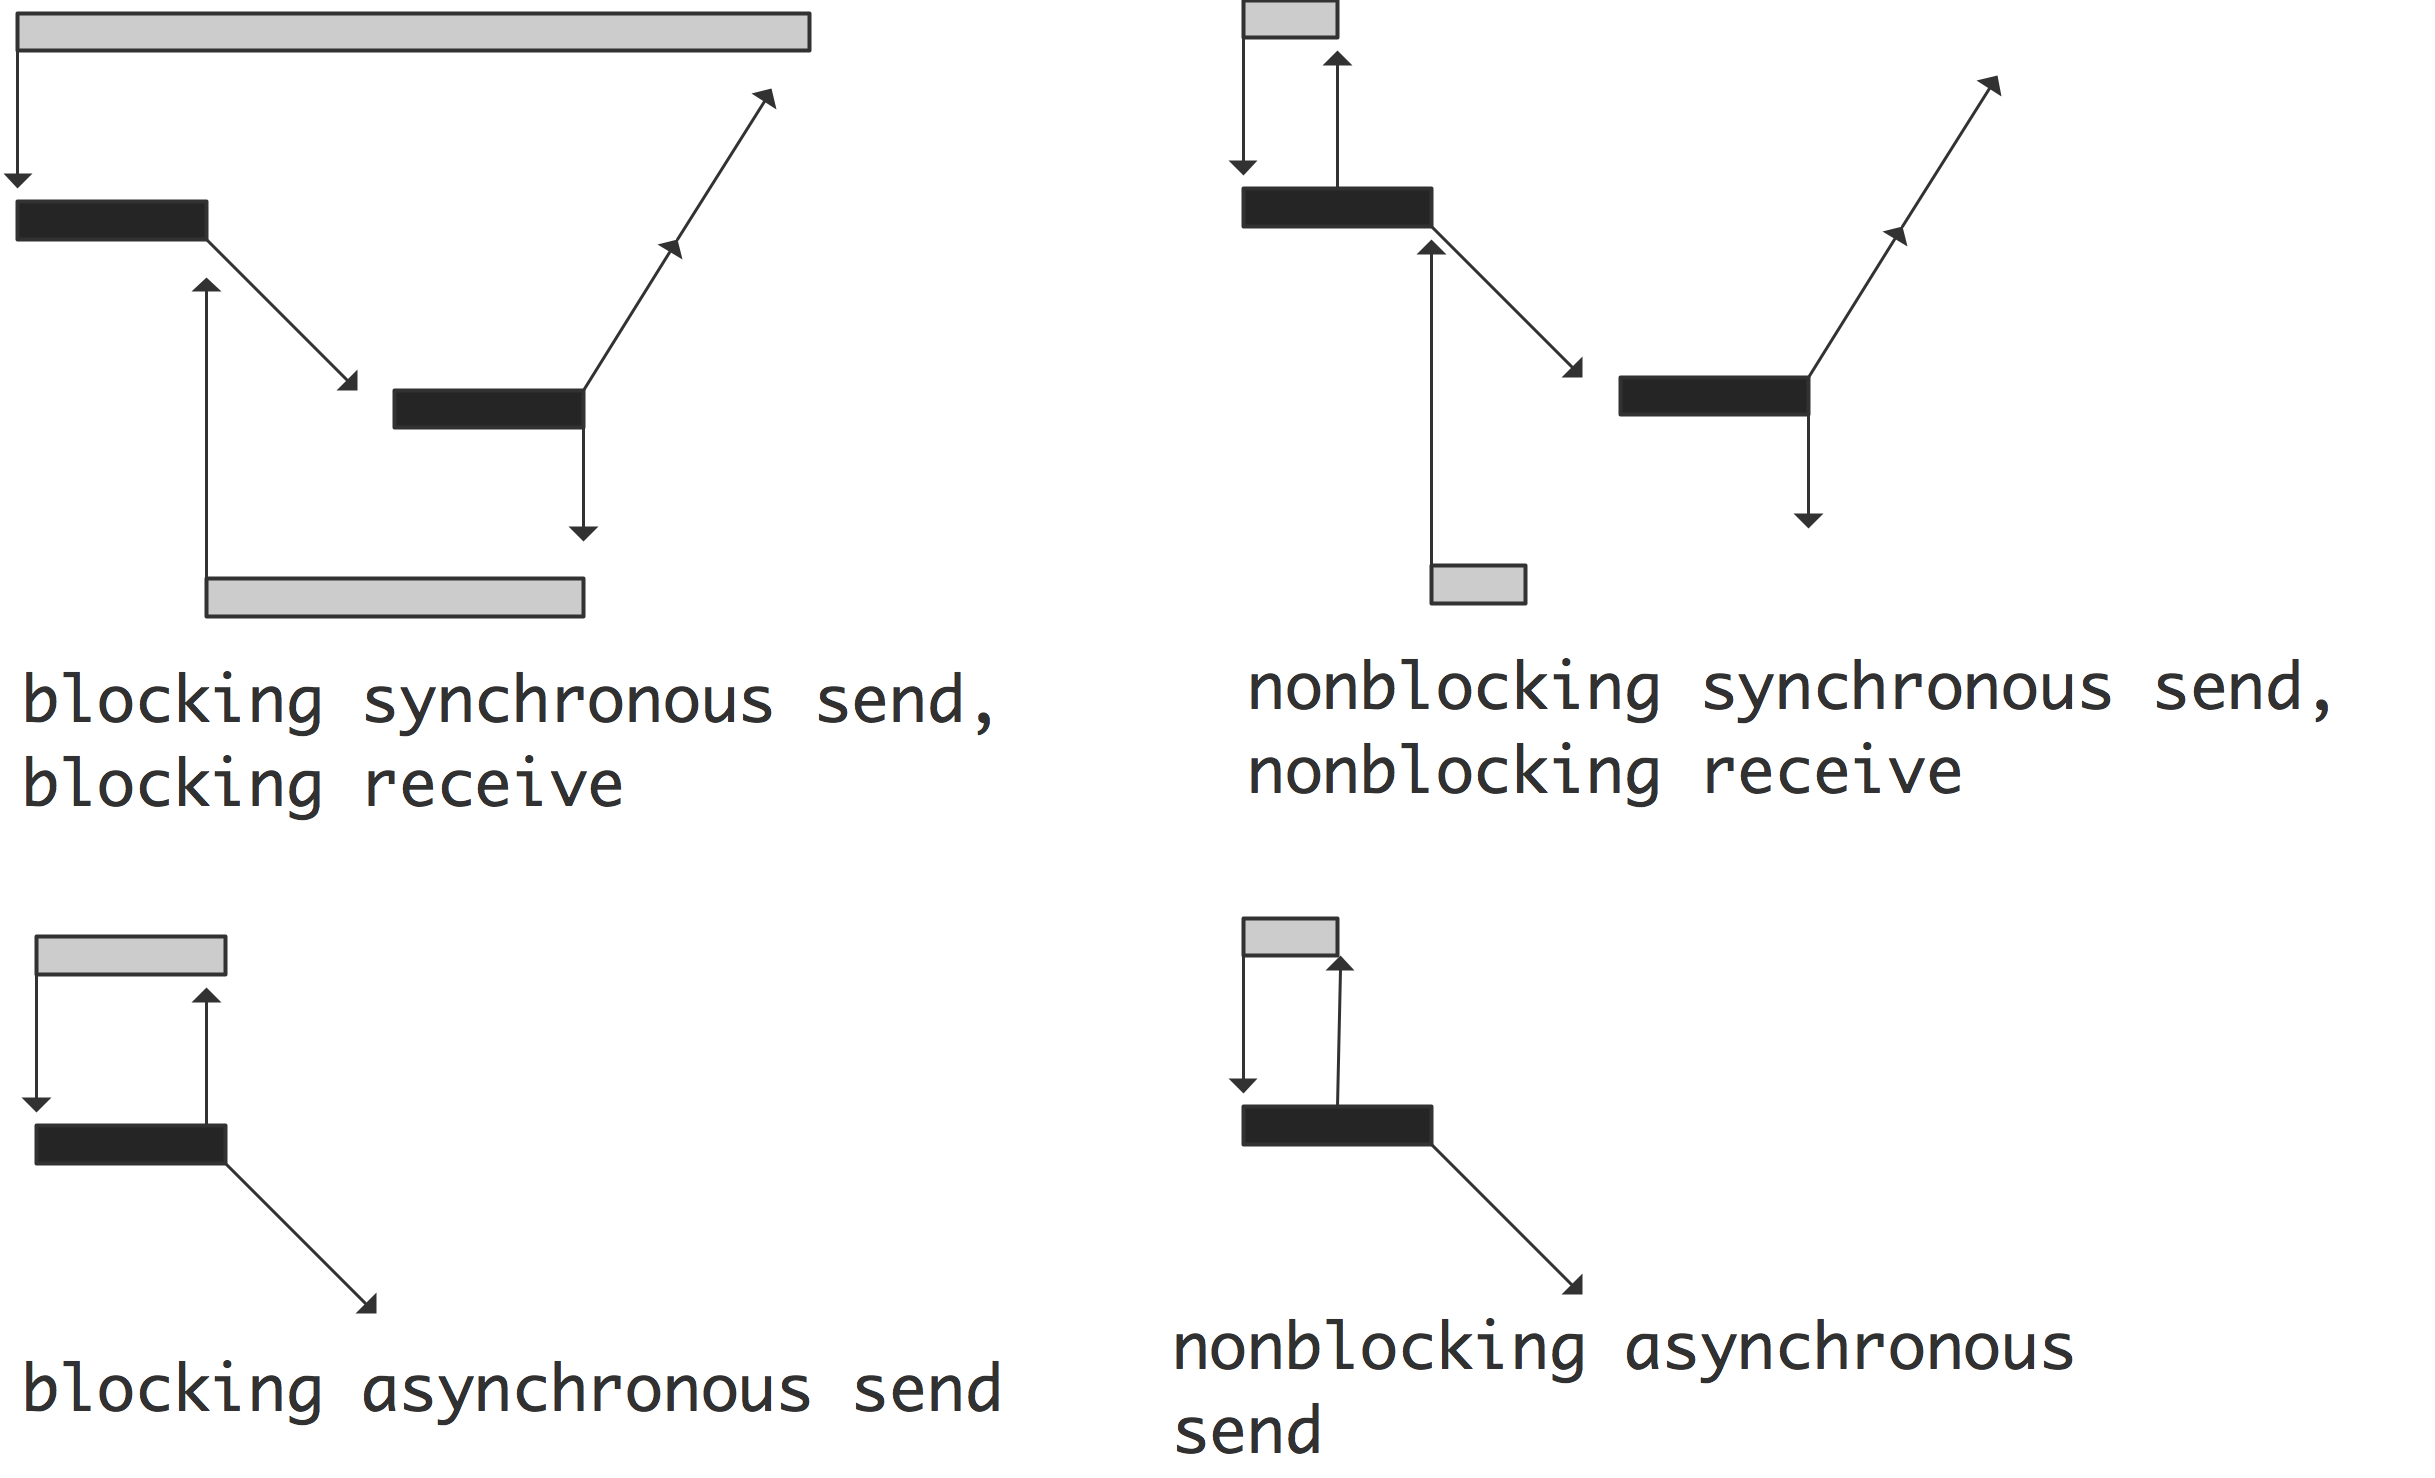
\includegraphics[scale=.15]{block-vs-sync}
\caption{Blocking and synchronicity}
\label{fig:block-sync}
\end{figure}
The four possible cases are illustrated in figure~\ref{fig:block-sync}.

\index{communication!synchronous|)}
\index{communication!asynchronous|)}

\Level 1 {Buffered communication}
\commandref{buffered}

By now you have probably got the notion that managing buffer
space in MPI is important: data has to be somewhere, either in
user-allocated arrays or in system buffers. Buffered sends are yet another
way of managing buffer space.
\begin{enumerate}
\item You allocate your own buffer space, and you attach it to your process;
\item You use the \indexmpishow{MPI_Bsend} call for sending;
\item You detach the buffer when you're done with the buffered sends.
\end{enumerate}

There can be only one buffer per process; its size should be enough
for all outstanding \indexmpishow{MPI_Bsend} calls that are simultaneously
outstanding, plus \indexmpishow{MPI_BSEND_OVERHEAD}.

\Level 1 {Persistent communication}
\commandref{persistent}
\index{communication!persistent|(textbf}

An \n{Isend} or \n{Irecv} call as an \n{MPI_Request} parameter. This
is an object that gets created in the send/recv call, and deleted in
the wait call. You can imagine that this carries some overhead, and if
the same communication is repeated many times you may want to avoid
this overhead by reusing the request object.

To do this, MPI has \emph{persistent communication}:
\index{persistent communication|see{communication, persistent}}
\begin{itemize}
\item You describe the communication with
  \indexmpishow{MPI_Send_init}, which has the same calling sequence as
  \n{MPI_Isend}, or \indexmpishow{MPI_Recv_init}, which has the same
  calling sequence as \n{MPI_Irecv}.
\item The actual communication is performed by calling
  \indexmpishow{MPI_Start}, for a single request, or
  \indexmpishow{MPI_Startall} for an array or requests.
\item Completion of the communication is confirmed with
  \indexmpishow{MPI_Wait} or similar routines as you have seen in the
  explanation of non-blocking communication.
\item The wait call does not release the request object: that is done
  with \indexmpishow{MPI_Request_free}.
\end{itemize}

\index{communication!persistent|)}

\index{communication!non-blocking|)}
\index{communication!two-sided|)}

\Level 1 {One-sided communication}
\commandref{one-sided}
\index{communication!one-sided|(}
\index{target!active synchronization|see{active target synchronization}}
\index{target!passive synchronization|see{passive target synchronization}}

Above, you saw  point-to-point operations of the two-sided type:
they require the co-operation of a sender and
receiver. This co-operation could be loose: you can post a receive
with \n{MPI_ANY_SOURCE} as sender, but there had to be both a send and
receive call. In this section, you will see one-sided communication 
routines where a process
can do a `put' or `get' operation, writing data to or reading it from
another processor, without that other processor's involvement.

In one-sided MPI operations, also known as \acf{RDMA} or 
\acf{RMA} operations, there
are still two processes involved: the \indexterm{origin}, which is the
process that originates the transfer, whether this is a `put' or a `get',
and the \indexterm{target} whose
memory is being accessed. Unlike with two-sided operations, the target
does not perform an action that is the counterpart of the action on the origin.

That does not mean that the origin can access arbitrary data on the target
at arbitrary times. First of all, one-sided communication in MPI
is limited to accessing only a specifically declared memory area on the target:
the target declares an area of
user-space memory that is accessible to other processes. This is known
as a \indexterm{window}. Windows limit how origin processes can access
the target's memory: you can only `get' data from a window or `put' it
into a window; all the other memory is not reachable from other processes.

The alternative to having windows is to use \indexterm{distributed shared memory}
or \indexterm{virtual shared memory}: memory is distributed but acts as if
it shared. The so-called \acf{PGAS} languages such as \ac{UPC} use this model.
The MPI \ac{RMA} model makes it possible to 
lock a window which makes programming slightly more cumbersome, but the
implementation more efficient.

Within one-sided communication, MPI has two modes: active RMA and
passive RMA. In \indextermsub{active}{RMA}, or \indexterm{active target synchronization},
the target sets boundaries on the time period (the `epoch')
during which its window can be accessed.
The main advantage
of this mode is that the origin program can perform many small transfers, which are
aggregated behind the scenes. Active RMA acts much like asynchronous transfer with a
concluding \n{Waitall}.

In \indextermsub{passive}{RMA}, or \indexterm{passive target synchronization},
the target process puts no limitation on when its window can be accessed.
(\ac{PGAS} languages such as \ac{UPC} are based on this model: data is 
simply read or written at will.)
While 
intuitively it is attractive to be able to write to and read from a target at
arbitrary time,
there are problems. For instance, it requires a remote agent on the target,
which may interfere with execution of the main thread, or conversely it may not be
activated at the optimal time. Passive RMA is also very hard to debug and can lead
to strange deadlocks.

%% McLaren says use an info object

\Level 2 {Windows}
\commandref{windows}
\index{window|(}

In one-sided communication, each processor can make an area of memory
available, called a \indexterm{window}. This has the following
characteristics:
\begin{itemize}
\item The window is defined on a communicator, so the create call
  is collective.
\item The window size can be set individually on each process.
  A~zero size is allowed, but since window creation is collective,
  it is not possible to skip the create call.
\end{itemize}
\begin{figure}[ht]
  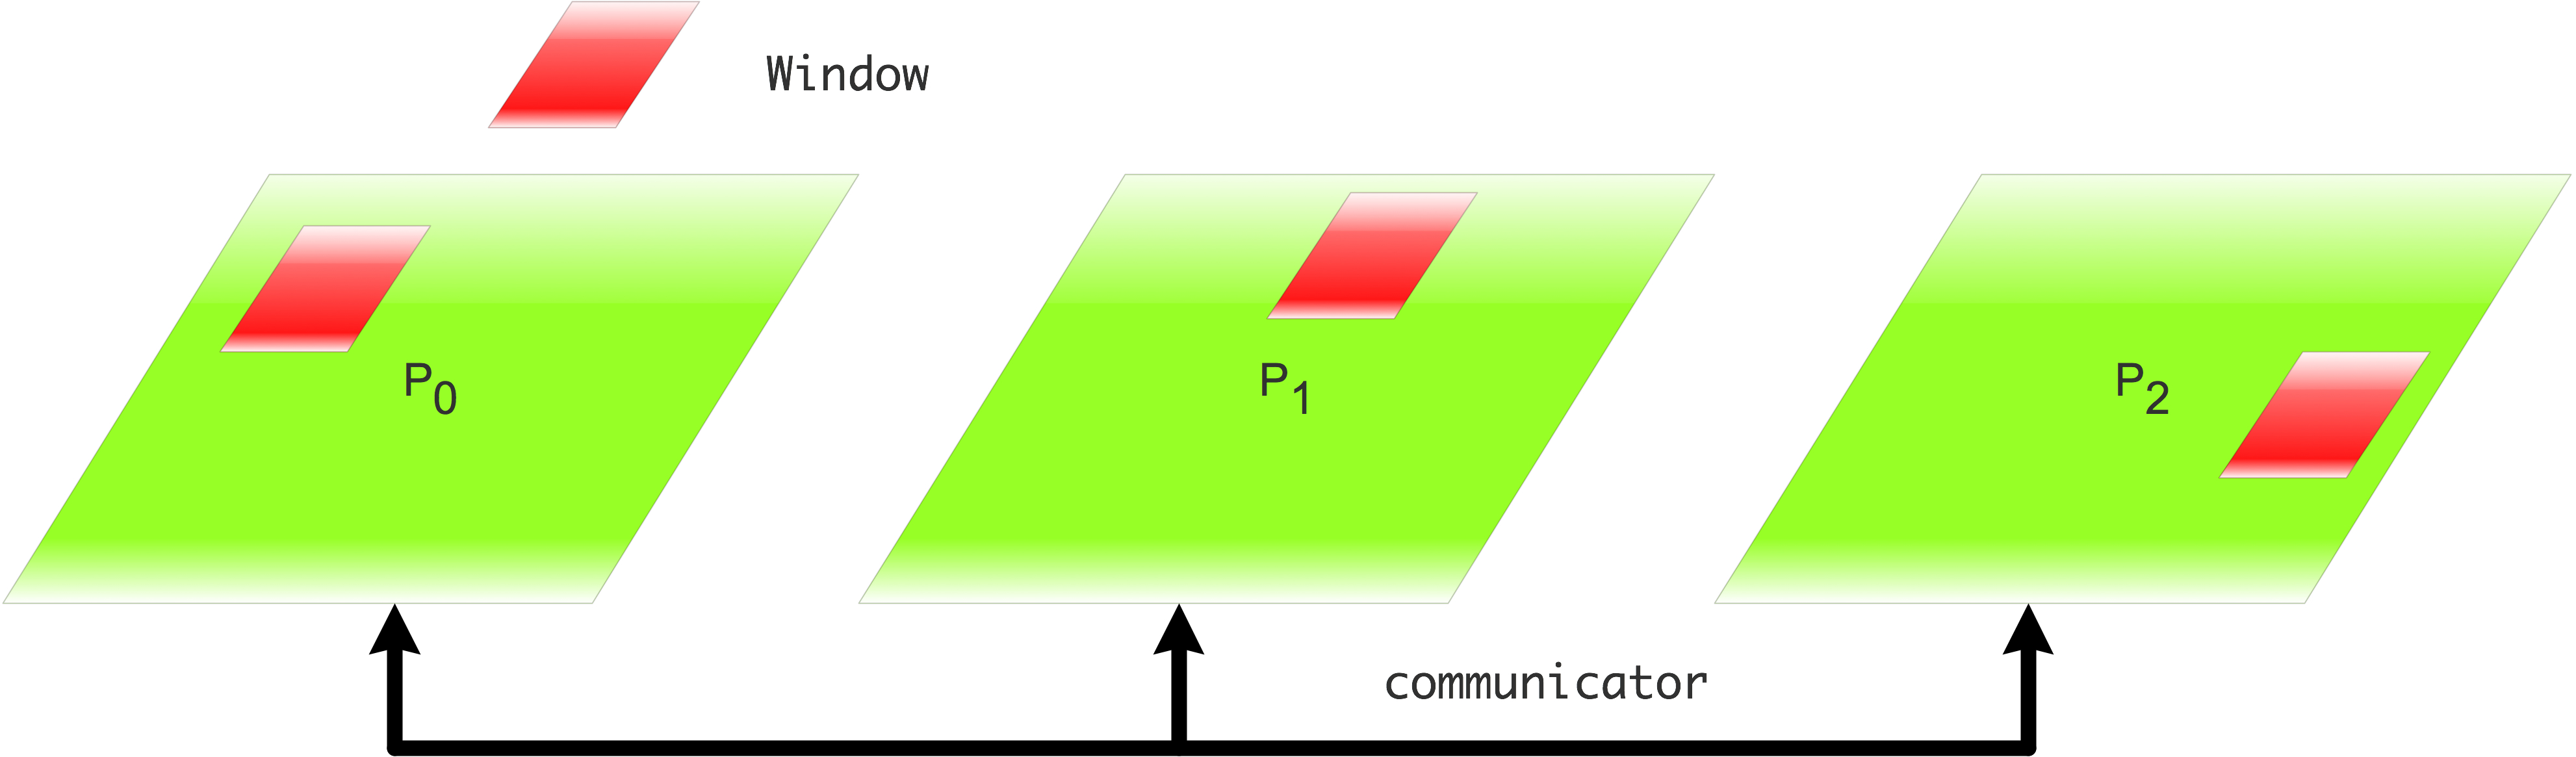
\includegraphics[scale=.1]{graphics/one-sided-window}
  \caption{Collective definition of a window for one-sided data access}
  \label{fig:window}
\end{figure}
defined with respect to a communicator: each process specifies a
memory area. Routine for creating and releasing windows
are collective, so each process \emph{has} to
call them; see figure~\ref{fig:window}. 
\begin{verbatim}
MPI_Info info;
MPI_Win window;
MPI_Win_create( /* memory area */, info, comm, &window );
MPI_Win_free( &window );
\end{verbatim}
(For the \n{info} parameter you can often use \indexmpishow{MPI_INFO_NULL}.)
While the creation of a window is collective, each
processor can specify its own window size, including zero, and even the type of the
elements in it.

The MPI specification allows that the memory of a window can be 
separate from the regular program memory. The routine \indexmpishow{MPI_Alloc_mem}
can return a pointer to such priviliged memory.

\begin{verbatim}
MPI_Info info ;
int error ;
error = MPI_Info_create ( & info ) ;
error = MPI_Info_set ( info , "no_locks" , "true" ) ;
/* Use the info object*/
error = MPI_Info_free ( info ) ;
\end{verbatim}

\Level 2 {Active target synchronization: epochs}
\commandref{fence}

There are two mechanisms for \indexterm{active target synchronization}, that is,
one-sided communications where both sides are involved to the extent that they declare
the communication epoch. In this section we look at the first mechanism,
which is to use a \indexterm{fence} operation:\indexmpi{MPI_Win_fence}
\begin{verbatim}
MPI_Win_fence (int assert, MPI_Win win)
\end{verbatim}
This operation is collective on the communicator of the window.
It is comparable to \n{MPI_Wait} calls for non-blocking communication.

The use of fences is somewhat complicated. The interval between two fences
is known as an \indexterm{epoch}.
You can give various hints to the system about this epoch versus the ones
before and after through the \n{assert} parameter.
\begin{verbatim}
MPI_Win_fence((MPI_MODE_NOPUT | MPI_MODE_NOPRECEDE), win);
MPI_Get( /* operands */, win);
MPI_Win_fence(MPI_MODE_NOSUCCEED, win);
\end{verbatim}
In between the two fences the window is exposed, and while it is you
should not access it locally. If you absolutely need to access it
locally, you can use an \ac{RMA} operation for that. Also, there can be only one
remote process that does a \n{put}; multiple \n{accumulate} accesses are allowed.

Fences are, together with other window calls, collective operations. That means they 
imply some amount of synchronization between processes. Consider:
\begin{verbatim}
MPI_Win_fence( ... win ... ); // start an epoch
if (mytid==0) // do lots of work
else // do almost nothing
MPI_Win_fence( ... win ... ); // end the epoch
\end{verbatim}
and assume that all processes execute the first fence more or less at the same time.
The zero process does work before it can do the second fence call, but all other
processes can call it immediately. However, they can not finish that second fence call
until all one-sided communication is finished, which means they wait for the zero process.
\begin{figure}[ht]
  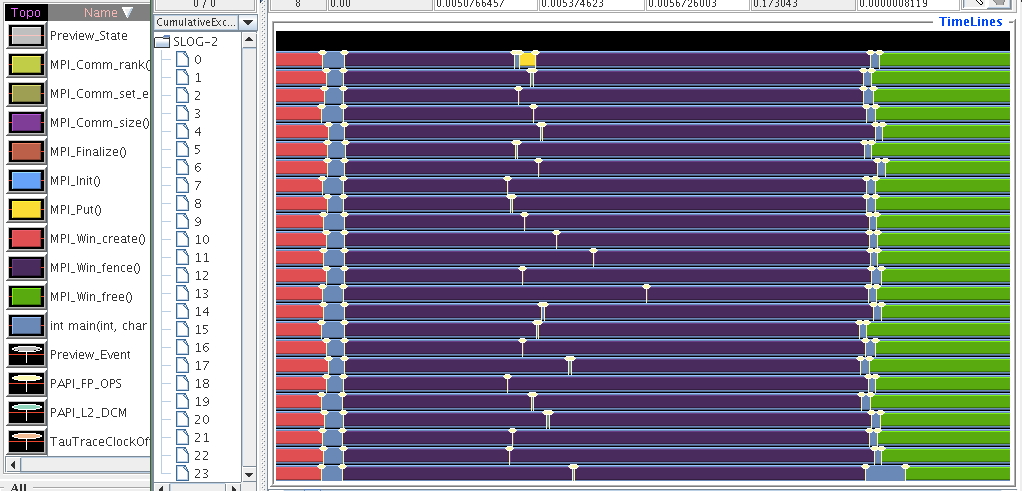
\includegraphics[scale=.4]{graphics/lonestar-twonode-put}%putblock
  \caption{A trace of a one-sided communication epoch where process zero only originates
  a one-sided transfer}
  \label{fig:putblock}
\end{figure}
\verbatimsnippet{putblock}

As a further restriction, you can not mix \n{Get} with \n{Put} or \n{Accumulate}
calls in a single epoch. Hence, we can characterize an epoch as an
\indextermsub{access}{epoch} on the origin, and
as an \indextermsub{exposure}{epoch} on the target.

Assertions are an integer parameter: you can add or logical-or values.
The value zero is always correct. There are two types of parameters.
Local assertions are:
\begin{itemize}
  \item\indexmpishow{MPI_MODE_NOSTORE} The preceding epoch did not store
    anything in this window.
  \item\indexmpishow{MPI_MODE_NOPUT} The following epoch will not store
    anything in this window.
\end{itemize}
Global assertions:
\begin{itemize}
  \item\indexmpishow{MPI_MODE_NOPRECEDE} This process made no \ac{RMA}
    calls in the preceding epoch.  
  \item\indexmpishow{MPI_MODE_NOSUCCEED} This process will make no
    \ac{RMA} calls in the next epoch.
\end{itemize}

\index{window|)}

\Level 2 {Put, get, accumulate}
\commandref{putget}

Window areas are 
accessible to other processes in the communicator by specifying the
process rank and an offset from the base of the window.\indexmpi{MPI_Put}
\begin{verbatim}
MPI_Put (
  void *origin_addr, int origin_count, MPI_Datatype origin_datatype,
  int target_rank,
  MPI_Aint target_disp, int target_count, MPI_Datatype target_datatype,
  MPI_Win window)
\end{verbatim}
The \indexmpishow{MPI_Get} call is very similar; a third one-sided routine
is \indexmpishow{MPI_Accumulate} which does a reduction operation on the results
that are being put:
\begin{verbatim}
MPI_Accumulate (
  void *origin_addr, int origin_count, MPI_Datatype origin_datatype, 
  int target_rank,
  MPI_Aint target_disp, int target_count, MPI_Datatype target_datatype,
  MPI_Op op,MPI_Win window)
\end{verbatim}

\begin{exercise}
  Implement an `all-gather' operation using one-sided communication:
  each processor stores a single number, and you want each processor
  to build up an array that contains the values from all
  processors. Note that you do not need a special case for a processor
  collecting its own value: doing `communication' between a processor
  and itself is perfectly legal.
\end{exercise}

Accumulate is a reduction with remote result. As with \n{MPI_Reduce}, the 
order in which the operands are accumulated is undefined. 
The same predefined operators are available, but no
user-defined ones. There is one extra operator: \indexmpishow{MPI_REPLACE},
this has the effect that only the last result to arrive is retained.

\Level 2 {Put vs Get}

\begin{verbatim}
while(!converged(A)){ 
  update(A); 
  MPI_Win_fence(MPI_MODE_NOPRECEDE, win); 
  for(i=0; i < toneighbors; i++) 
    MPI_Put(&frombuf[i], 1, fromtype[i], toneighbor[i], 
                         todisp[i], 1, totype[i], win); 
  MPI_Win_fence((MPI_MODE_NOSTORE | MPI_MODE_NOSUCCEED), win); 
  } 
\end{verbatim}
\begin{verbatim}
  while(!converged(A)){ 
  update_boundary(A); 
  MPI_Win_fence((MPI_MODE_NOPUT | MPI_MODE_NOPRECEDE), win); 
  for(i=0; i < fromneighbors; i++) 
    MPI_Get(&tobuf[i], 1, totype[i], fromneighbor[i], 
                    fromdisp[i], 1, fromtype[i], win); 
  update_core(A); 
  MPI_Win_fence(MPI_MODE_NOSUCCEED, win); 
  } 
\end{verbatim}

\Level 2 {More active target synchronization}
\commandref{post-wait}

There is a more fine-grained ways of doing 
\indexterm{active target synchronization}. While fences
corresponded to a global synchronization of one-sided calls,
the \n{MPI_Win_start},
\n{MPI_Win_complete}, \n{MPI_ Win_post}, \n{Win_wait} routines
are suitable, and possibly more efficient,
if only a small number of processor pairs is
involved.  Which routines
you use depends on whether the processor is an \indexterm{origin} or
\indexterm{target}.

If the current process is going to have the data in its window accessed,
you define an \indextermsub{exposure}{epoch} by:
\begin{verbatim}
MPI_Win_post( /* group of origin processes */ )
MPI_Win_wait()
\end{verbatim}
This turns the current processor into a target for access operations issued
by a different process.

If the current process is going to be issuing one-sided operations,
you define an \indextermsub{access}{epoch} by:
\begin{verbatim}
MPI_Win_start( /* group of target processes */ )
// access operations
MPI_Win_complete()
\end{verbatim}
This turns the current process into the origin of a number of
one-sided access operations.

Both pairs of operations declare a
\indextermbus{group of}{processors}; see section~\ref{sec:comm-group}
for how to get such a group from a communicator.
On an origin processor you would specify a group that includes the targets
you will interact with, on a target processor you specify a group
that includes the possible origins.

\Level 2 {Passive target synchronization}
\commandref{passive-sync}

In \indexterm{passive target synchronization} only the origin is
actively involved: the target makes no calls whatsoever.
This means that the origin process remotely locks the window
on the target.

During an access epoch, a process can initiate and finish a one-sided
transfer.
\begin{verbatim}
If (rank == 0) {
  MPI_Win_lock (MPI_LOCK_EXCLUSIVE, 1, 0, win);
  MPI_Put (outbuf, n, MPI_INT, 1, 0, n, MPI_INT, win);
  MPI_Win_unlock (1, win);
}
\end{verbatim}
The two lock types are:
\begin{itemize}
\item \indexmpishow{MPI_LOCK_SHARED} which should be used for \n{Get}
  calls: since multiple processors are allowed to read from a window
  in the same epoch, the lock can be shared.
\item \indexmpishow{MPI_LOCK_EXCLUSIVE} which should be used for
  \n{Put} and \n{Accumulate} calls: since only one processor is
  allowed to write to a window during one epoch, the lock should be
  exclusive.
\end{itemize}
These routines make MPI behave like a shared memory system; the
instructions between locking and unlocking the window effectively
become \indexterm{atomic operations}.

The above mechanism is of limited use.
Suppose processor zero has a data structure \n{work_table}
with items that need to be processed. A~counter \n{first_work}
keeps track of the lowest numbered item that still needs processing.
You can imagine the following
\indexterm{master-worker} scenario:
\begin{itemize}
\item Each process connects to the master,
\item inspects the \n{first_work} variable,
\item retrieves the corresponding work item, and
\item increments the \n{first_work} variable.
\end{itemize}
It is important here to avoid a \indexterm{race condition}
(see section \HPSCref{sec:shared-lock}) that would result
from a second process reading the \n{first_work} variable 
before the first process could have updated it. Therefore, the reading
and updating needs to be an \indexterm{atomic operation}.

Unfortunately, you can not have a put and get call in the same access
epoch. For this reason, MPI version~3 has added certain atomic
operations, such as \indexmpishow{MPI_Fetch_and_op}.

\Level 2 {Details}
\label{sec:mpi-alloc}

Sometimes an architecture has memory that is shared between processes,
or that otherwise is fast for one-sided communication. To put a window
in such memory, it can be placed in memory that is especially
allocated:
\begin{verbatim}
MPI_Alloc_mem() and MPI_Free_mem()
\end{verbatim}
These calls reduce to \n{malloc} and \n{free} if there is no special
memory area; SGI is an example where such memory does exist.

\Level 2 {Implementation}
\index{communication!one-sided, implementation of|(}

You may wonder how one-sided communication is realized\footnote{For
  more on this subject, see~\cite{thakur:ijhpca-sync}.}. Can a processor
somehow get at another processor's data? Unfortunately, no.

Active target synchronization is implemented in terms of two-sided communication.
Imagine that the first fence operation does nothing, unless it concludes prior
one-sided operations. The Put and Get calls do nothing involving communication,
except for marking with what processors they exchange data.
The concluding fence is where everything happens: first a global operation
determines which targets need to issue send or receive calls, then the
actual sends and receive are executed.

\begin{exercise}
  Assume that only Get operations are performed during an epoch. 
  Sketch how these are translated to send/receive pairs. 
  The problem here is how the senders find out that they need to send.
  Show that you can solve this with an \indexmpishow{MPI_Scatter_reduce} call.
\end{exercise}

The previous paragraph noted that a collective operation was necessary
to determine the two-sided traffic. Since collective operations induce
some amount of synchronization, you may want to limit this.

\begin{exercise}
  Argue that the mechanism with window post/wait/start/complete operations
  still needs a collective, but that this is less burdensome.
\end{exercise}

Passive target synchronization needs another mechanism entirely.  Here
the target process needs to have a background task (process, thread,
daemon,\ldots) running that listens for requests to lock the
window. This can potentially be expensive.

\index{communication!one-sided, implementation of|)}
\index{communication!one-sided|)}

\Level 1 {Remaining topics in point-to-point communication}

\Level 2 {Subtleties with processor synchronization}
\label{sec:handshake}

Blocking communication involves a complicated dialog between the two
processors involved. Processor one says `I~have this much data to
send; do you have space for that?', to which processor two replies
`yes, I~do; go ahead and send', upon which processor one does the
actual send. This back-and-forth (technically known as
a \indexterm{handshake}) takes a certain amount of communication
overhead. For this reason, network hardware will sometimes forgo the
handshake for small messages, and just send them regardless, knowing
that the other process has a small buffer for such occasions.

%This behaviour is not dictated by the standard: it is up to the implementation
%to make this optimization for small messages.

One strange side-effect of this strategy is that a code that
should \indexterm{deadlock} according to the MPI specification does
not do so. In effect, you may be shielded from you own programming
mistake! Of course, if you then run a larger problem, and the small
message becomes larger than the threshold, the deadlock will suddenly
occur. So you find yourself in the situation that a bug only manifests
itself on large problems, which are usually harder to debug. In this
case, replacing every \n{MPI_Send} with a \indexmpishow{MPI_Ssend} will force the
handshake, even for small messages.

Conversely, you may sometimes wish to avoid the handshake on large
messages. MPI as a solution for this: the \indexmpishow{MPI_Rsend} (`ready
send') routine sends its data immediately, but it needs the receiver
to be ready for this. How can you guarantee that the receiving process
is ready? You could for instance do the following (this uses
non-blocking routines, which are explained below in
section~\ref{sec:nonblocking}):
\begin{verbatim}
if ( receiving ) {
  MPI_Irecv()   // post non-blocking receive
  MPI_Barrier() // synchronize
else if ( sending ) {
  MPI_Barrier() // synchronize
  MPI_Rsend()   // send data fast
\end{verbatim}
When the barrier is reached, the receive has been posted, so it is safe 
to do a ready send. However, global barriers are not a good idea.
Instead you would just synchronize the two processes involved.
\begin{exercise}
  Give pseudo-code for a scheme where you synchronize the two
  processes through the exchange of a blocking zero-size message.
\end{exercise}

\Level 2 {The origin of one-sided communication in ShMem}

The \indextermbus{Cray}{T3E} had a library called \indexterm{shmem}
which offered a type of shared memory. Rather than having a true
global address space it worked by supporting variables that were
guaranteed to be identical between processors, and indeed, were
guaranteed to occupy the same location in memory. Variables could be
declared to be shared a `symmetric' pragma or directive; their values
could be retrieved or set by \n{shmem_get} and \n{shmem_put} calls.

